% ARPEGOS:  Automatized Roleplaying-game Profile Extensible Generator Ontology based System %
% Author : Alejandro Muñoz Del Álamo %
% Copyright 2019 %

% Section 11.1: Objetivos alcanzados %
\section{Funcionamiento de \protege}
En esta sección se describe cómo debe utilizarse \protege para crear los diferentes elementos que componen una nueva ontología,
de tal manera que pueda ser utilizada por la aplicación de este proyecto. Para ello, recordamos que los elementos subrayados 
deben utilizarse exactamente como están indicados en el manual. Todas las capturas que se muestran en esta sección forman 
parte del proceso de creación de la ontología de \anima. 

\subsection{Ontología}
\subsubsection{Configurar ontología}
El primer paso para elaborar una ontología para \textit{ARPEGOS} es crear un fichero con formato \textit{OWL} en el que 
se detalle la información de la ontología. Esto se hace de la siguiente manera: 

\begin{enumerate}
    
    \item En primer lugar, cuando se abre la aplicación \protege, ésta se inicia como si fuera a crear una ontología nueva. En 
    caso de estar trabajando con una ontología y querer crear una nueva, basta con ir a \textit{File} - \textit{New} (figura \ref*{Create_new_ontology}) o utilizar 
    el atajo de teclado \textit{Ctrl + N}.

    \begin{figure}[H]
        \centering
        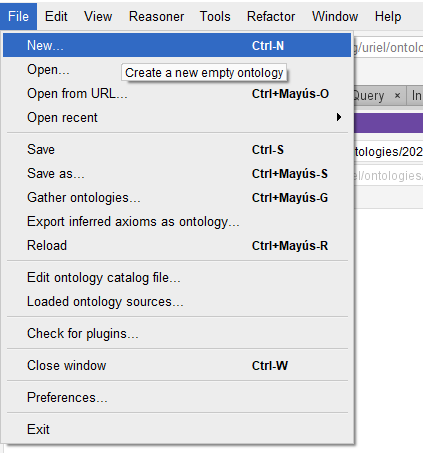
\includegraphics[scale=0.6]{Figures/Protege/Create_Ontology.png}
        \caption{Paso 1: Crear una nueva ontología}
        \label{Create_new_ontology}
    \end{figure}

    \item Una vez estamos en la pantalla de inicio de la nueva ontología, hay que editar los campos \textit{Ontology IRI} y 
    \textit{Ontology Version IRI}. Estos campos deben rellenarse de una manera específica, tal y como se muestra en la 
    figura \ref*{IRI_demo}:

    \begin{figure}[ht]
        \centering
        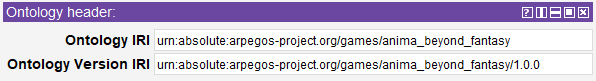
\includegraphics[scale=0.6]{Figures/Protege/IRI_demo.png}
        \caption{Campos \textit{IRI} de la ontología de \anima}
        \label{IRI_demo}
    \end{figure}

    \newpage
    El \textit{Ontology IRI} debe tener la misma raíz para todas las ontologías:

    \textit{\underline{urn:absolute:arpegos-project.org/games/}nombre\_RPG} \medskip

    En el caso del \textit{Ontology Version IRI}, basta con copiar el \textit{Ontology IRI} y añadir al final el numero de versión 
    separado por una barra.\medskip

    \item Ahora sólo queda añadir las anotaciones que aportan información sobre la ontología, tales como su nombre, su descripción, su
    creador o creadores, y los derechos sobre la misma. Esto se puede apreciar en la figura \ref*{anima_annotations}.

    \begin{figure}[ht]
        \centering
        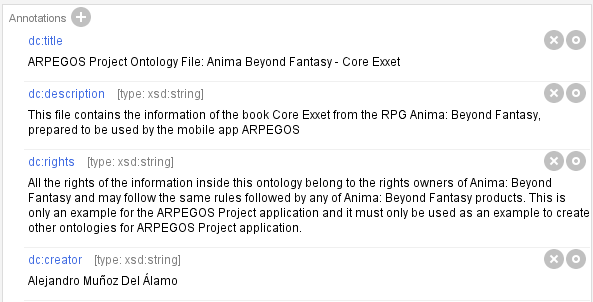
\includegraphics[scale=0.6]{Figures/Protege/anima_annotations.png}
        \caption{Campos \textit{IRI} de la ontología de \anima}
        \label{anima_annotations}
    \end{figure}
\end{enumerate}

\subsection{Anotaciones}
\subsubsection{Crear una anotación}
Para hacer cualquier anotación hay que seguir los siguientes pasos:

\begin{enumerate}
    \item Seleccionar el elemento al que se le desea añadir una anotación.
    \item Pulsar el botón “+” en el campo de anotaciones (Figura \ref*{annotation_1}).
    \begin{figure}[H]
        \centering
        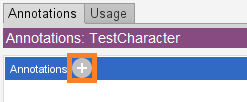
\includegraphics[scale=0.6]{Figures/Protege/Annotations.png}
        \caption{Pulsar el botón “+” en el campo de anotaciones}.
        \label{annotation_1}
    \end{figure}

    \item Seleccionar uno de los tipos de anotaciones en el campo izquierdo (Figura \ref*{annotation_2})
    \begin{figure}[H]
        \centering
        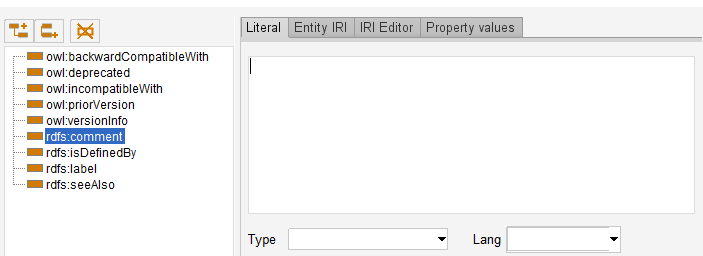
\includegraphics[scale=0.6]{Figures/Protege/Annotations_1.png}
        \caption{Seleccionar tipo de anotación}.
        \label{annotation_2}
    \end{figure}

    \item Introducir valor de la anotación en el campo derecho (Figura \ref*{annotation_3})
    \begin{figure}[H]
        \centering
        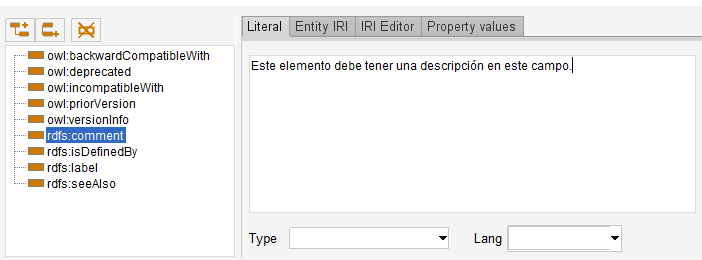
\includegraphics[scale=0.6]{Figures/Protege/Annotations_2.png}
        \caption{Introducir valor de anotación}.
        \label{annotation_3}
    \end{figure}

    \item Seleccionar tipo de datos de la anotación (Figura \ref*{annotation_4})
    \begin{figure}[H]
        \centering
        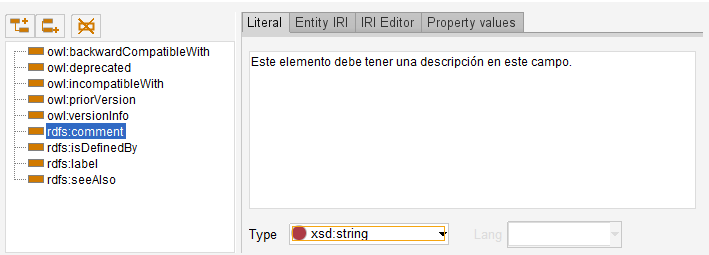
\includegraphics[scale=0.6]{Figures/Protege/Annotations_3.png}
        \caption{Seleccionar tipo de datos de la anotación}.
        \label{annotation_4}
    \end{figure}

    \item Pulsar el botón \textit{Aceptar}.
\end{enumerate}

\subsubsection{Crear un tipo de anotación personalizado}
Para el correcto funcionamiento de la aplicación son necesarias algunas anotaciones personalizadas. Esto es lo que 
hay que hacer para poder introducirlas en la aplicación:

\begin{enumerate}
    \item Acceder a la opción \textit{Annotation properties} de la vista \textit{Entities}.
    \item Seleccionar una anotación de la jerarquía y pulsar el botón \textit{Add sibling property}
    (Figura \ref*{CustomAnnotations_1}).
    \begin{figure}[H]
        \centering
        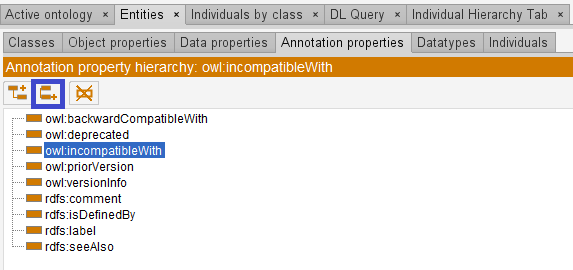
\includegraphics[scale=0.6]{Figures/Protege/CustomAnnotations_1.png}
        \caption{Seleccionar tipo de datos de la anotación}.
        \label{CustomAnnotations_1}
    \end{figure}
    \item Introducir el nombre del nuevo tipo de anotación y pulsar el botón \textit{Aceptar}.
\end{enumerate}

Las anotaciones personalizadas necesarias en la ontología para que el sistema de este proyecto pueda 
funcionar correctamente se muestran en la figura \ref*{Custom_Annotation_Types}:

\begin{figure}[ht]
    \centering
    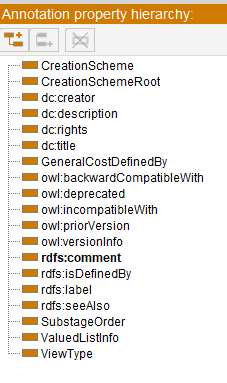
\includegraphics[scale=0.6]{Figures/Protege/Custom_Annotation_Types.png}
    \caption{Tipos de anotación utilizados en \textit{ARPEGOS}}.
    \label{Custom_Annotation_Types}
\end{figure}

\begin{itemize}
    \item \underline{dc:title}: Indica el nombre de la ontología.
    \item \underline{dc:description}: Indica la descripción de la ontología.
    \item \underline{dc:creator}: Indica el/los creador/es de la ontología.
    \item \underline{dc:rights}: Muestra los derechos de la ontología.
    \item \underline{CreationSchemeRoot}: Indica cual es la etapa raíz de creación
    \item \underline{CreationScheme}: Indica el orden del proceso de creación en la etapa raíz.
    \item \underline{GeneralCostDefinedBy}: Indica qué elemento define el coste general de una etapa.
    \item \underline{SubstageOrder}: Indica el orden de una subetapa.
    \item \underline{ValuedListInfo}: Define los elementos y cálculos necesarios para una etapa de asignación de valores.
    \item \underline{ViewType}: Indica el tipo de vista de la etapa asociada.
\end{itemize}

\subsection{Clases}
\subsubsection{Crear una clase o subclase} \label{CreateSubclass}
Una vez que ya se han establecido las propiedades de la ontología, es hora de empezar a añadir información a la misma.
Para ello, el primer paso es crear una clase. Una clase es un conjunto de elementos que poseen el mismo tipo de propiedades 
y características similares. Algunos ejemplos de clase son:
\begin{itemize}
    \item Raza del personaje (elfo, mediano, enano, orco, etc.)
    \item Habilidades del personaje (ataque, defensa, poderes mágicos, poderes psíquicos, etc.)
    \item Clase del personaje (paladín, guerrero, mago, ladrón, etc.)
\end{itemize}

En este ejemplo, vamos a crear la clase \textit{Raza} para representar las diferentes razas que hay en \anima.
Los pasos son los siguientes: 

\begin{enumerate}
    \item Acceder a la sección \textit{Entities}.
    \item Ir al apartado \textit{Classes}.
    \item Seleccionar la clase \textit{owl:Thing} en la jerarquía de clases (Figura \ref*{CreateClass_1}). En el caso de 
    querer crear una subclase a otra ya creada, seleccionar la clase que se desea utilizar como clase padre.
    \begin{figure}[H]
        \centering
        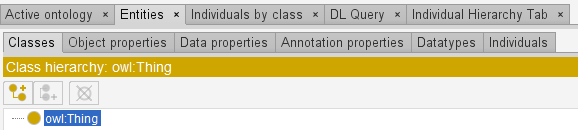
\includegraphics[scale=0.6]{Figures/Protege/CreateClass_1.png}
        \caption{Seleccionar la clase \textit{owl:Thing}}
        \label{CreateClass_1}
    \end{figure}
    
    \item Pulsar el botón \textit{Add subclass} (Figura \ref*{CreateClass_2}).
    
    \begin{figure}[ht]
        \centering
        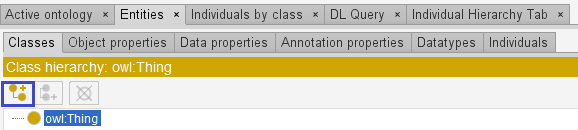
\includegraphics[scale=0.6]{Figures/Protege/CreateClass_2.png}
        \caption{Seleccionar la clase \textit{owl:Thing}}
        \label{CreateClass_2}
    \end{figure}

    \item Introducir el nombre de la clase. Como se puede observar en la figura \ref*{CreateClass_3}, el programa genera 
    el \textit{IRI} de la clase añadiendo su nombre tras la almohadilla. Además, si introducimos un nombre con espacios, 
    \protege sustituirá los espacios por guiones bajos.

    \begin{figure}[H]
        \centering
        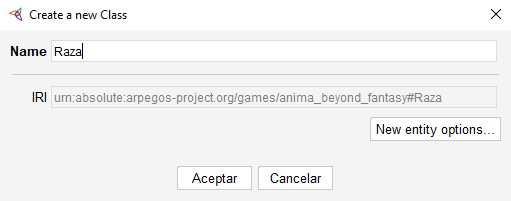
\includegraphics[scale=0.6]{Figures/Protege/CreateClass_3.png}
        \caption{Introducir el nombre de la clase}
        \label{CreateClass_3}
    \end{figure}

    \item Por último, hay que introducir una anotación del tipo \textit{\underline{rdfs:comment}} con la descripción 
    de la clase (figura \ref*{CreateClass_4}).

    \begin{figure}[ht]
        \centering
        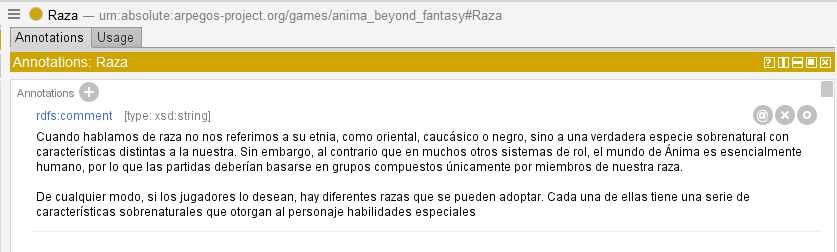
\includegraphics[scale=0.6]{Figures/Protege/CreateClass_4.png}
        \caption{Introducir descripción de la clase}
        \label{CreateClass_4}
    \end{figure}

\end{enumerate}

\subsubsection{Crear una clase hermana} \label{CreateSiblingClass}
En \anima, hay dos tipos de raza: las razas puras y las razas llamadas \textit{Nephilim}. Cada tipo de raza 
corresponde a una subclase de \textit{Raza}. Para crear la primera, es necesario crear una subclase de \textit{Raza}, 
pero es posible crear una clase hermana de \textit{Raza pura} de una manera distinta. Para ello, es necesario disponer 
de una clase de la misma altura jerárquica, por lo que se considerará que se ha creado la clase \textit{Raza Pura} siguiendo 
los pasos del apartado \nameref{CreateSubclass}.

\begin{enumerate}

    \item Seleccionar una clase del mismo nivel jerárquico que aquella que se desea crear (Figura \ref*{CreateClass_5}).
    
    \begin{figure}[ht]
        \centering
        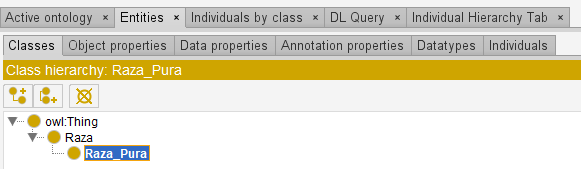
\includegraphics[scale=0.6]{Figures/Protege/CreateClass_5.png}
        \caption{Seleccionar una clase del nivel jerárquico deseado}
        \label{CreateClass_5}
    \end{figure}

    \item Pulsar el botón \textit{Add a sibling class} (Figura \ref*{CreateClass_6}).

    \begin{figure}[ht]
        \centering
        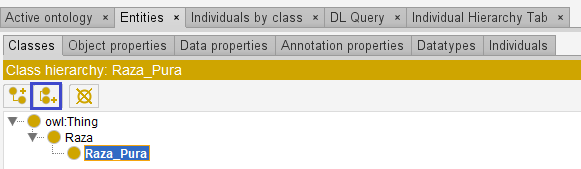
\includegraphics[scale=0.6]{Figures/Protege/CreateClass_6.png}
        \caption{Pulsar el botón \textit{Add a sibling class}}
        \label{CreateClass_6}
    \end{figure}

    \item Introducir el nombre de la clase (Figura \ref*{CreateClass_7}).
    
    \begin{figure}[ht]
        \centering
        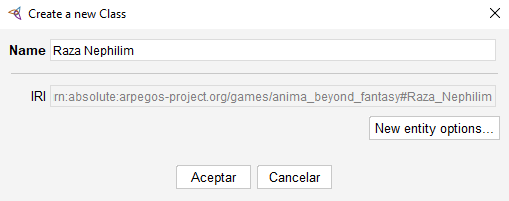
\includegraphics[scale=0.6]{Figures/Protege/CreateClass_7.png}
        \caption{Introducir el nombre de la clase hermana}
        \label{CreateClass_7}
    \end{figure}

    \item Incluir las anotaciones de la clase (Figura \ref*{CreateClass_8}).
    
    \begin{figure}[ht]
        \centering
        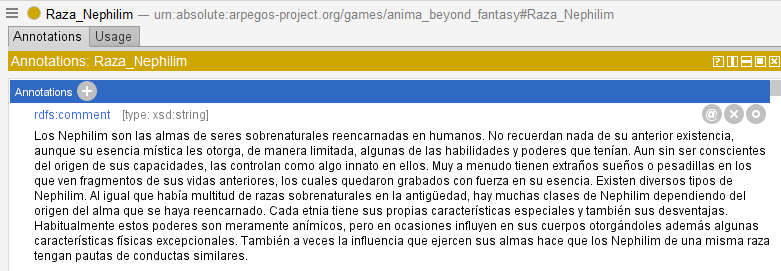
\includegraphics[scale=0.6]{Figures/Protege/CreateClass_8.png}
        \caption{Introducir la descripción de la clase hermana}
        \label{CreateClass_8}
    \end{figure}
\end{enumerate}

Para conseguir una mayor eficiencia en las búsquedas, se recomienda a los desarrolladores que indiquen qué clases son 
estrictamente distintas mediante el uso de la propiedad \textit{Disjoint with}. Para ello, basta con hacer lo siguiente:

\begin{enumerate}
    \item Pulsar sobre el símbolo “+” que se encuentra a la altura de \textit{Disjoint with} (Figura \ref*{CreateClass_9}).
    \begin{figure}[ht]
        \centering
        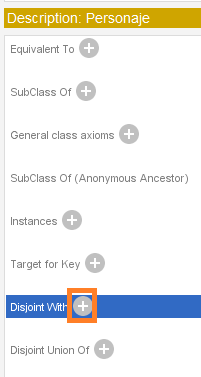
\includegraphics[scale=0.6]{Figures/Protege/CreateClass_9.png}
        \caption{Pulsar sobre el símbolo “+” de \textit{Domains (intersection)}}
        \label{CreateClass_9}
    \end{figure}

    \item Seleccionar la clase estrictamente distinta a la clase actual. Para ello, basta con navegar por la 
    jerarquía que se muestra en la ventana emergente (Figura \ref*{CreateClass_10}), elegir la clase correspondiente 
    y pulsar el botón \textit{Aceptar}.

    \begin{figure}[ht]
        \centering
        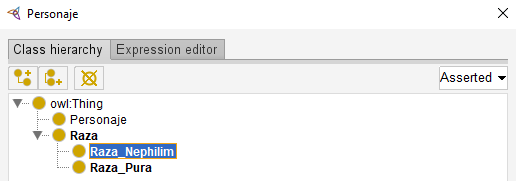
\includegraphics[scale=0.6]{Figures/Protege/CreateClass_10.png}
        \caption{Seleccionar clase de dominio}
        \label{CreateClass_10}
    \end{figure}

    Así, las clases pueden diferenciarse entre sí, tal y como se puede apreciar en la figura \ref*{CreateClass_11}
    \begin{figure}[ht]
        \centering
        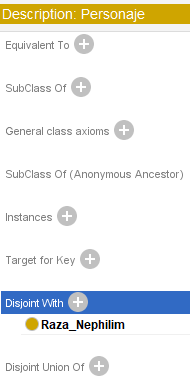
\includegraphics[scale=0.6]{Figures/Protege/CreateClass_11.png}
        \caption{Seleccionar clase de dominio}
        \label{CreateClass_11}
    \end{figure}
\end{enumerate}

\subsubsection{Eliminar clase de la ontología}
Al igual que es posible añadir clases a la ontología, es posible eliminarlas en caso de que haya algún error con alguna clase, o 
simplemente ésta sea prescindible.

\begin{enumerate}
    \item Seleccionar la clase que se desee eliminar (Figura \ref*{DeleteClass_1}).
    \begin{figure}[ht]
        \centering
        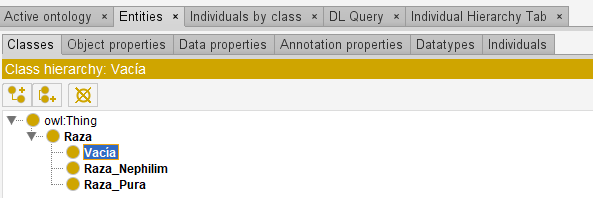
\includegraphics[scale=0.6]{Figures/Protege/DeleteClass_1.png}
        \caption{Seleccionar la clase a eliminar}
        \label{DeleteClass_1}
    \end{figure}

    \item Pulsar el botón \textit{Delete class} (Figura \ref*{DeleteClass_2}).
    \begin{figure}[ht]
        \centering
        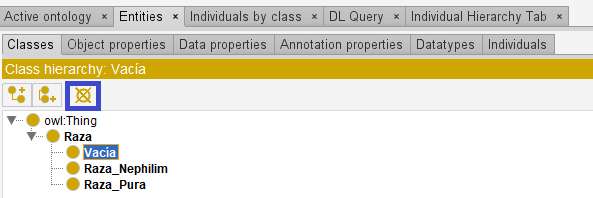
\includegraphics[scale=0.6]{Figures/Protege/DeleteClass_2.png}
        \caption{Pulsar el botón \textit{Delete class}}
        \label{DeleteClass_2}
    \end{figure}
\end{enumerate}

\subsection{Propiedades}
Uno de los puntos favorables de \protege es que una vez se conoce la forma de crear y eliminar clases, los procesos de creación y 
eliminación de las propiedades son exactamente iguales, de manera que se pueden seguir los mismos pasos en el apartado correspondiente 
de la pestaña \textit{Entities}. Los elementos que cambian son los elementos que se muestran en las vistas 
\textit{Characteristics} y \textit{Description} de las propiedades. \medskip

Una de las recomendaciones que propone el equipo de desarrollo es crear una jerarquía lógica para las propiedades, de manera que 
se puedan trabajar con ellas de la misma forma que con las clases. Esto facilitará una estructura lógica que posibilite una 
mayor mantenibilidad y legibilidad para desarrolladores y colaboradores.\medskip 

\textit{\textbf{Nota Importante}}: Como el objetivo de la aplicación es la creación de personajes, debe existir en la ontología 
un individuo que represente a un personaje de un jugador del juego, de manera que se puedan configurar correctamente las 
propiedades relacionadas con los personajes. Para esto hace falta crear una clase \textit{Personaje}, a la que pertenecerán los 
personajes creados con la aplicación. Como se muestra en la figura \ref*{CharacterClass}, para la ontología de \anima, se han 
creado varias subclases de personaje, en función del tipo de personaje que se desee crear.

\begin{figure}[ht]
    \centering
    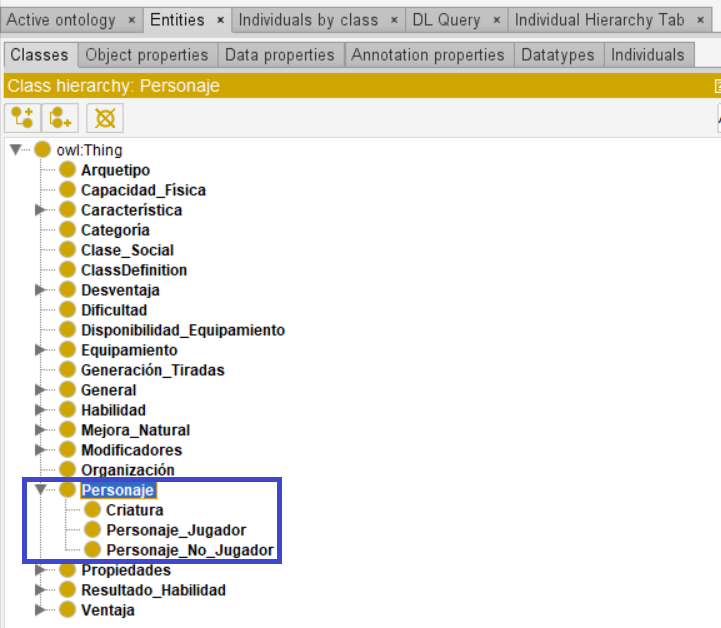
\includegraphics[scale=0.4]{Figures/Protege/CharacterClass.png}
    \caption{Clases que representan los diferentes tipos de personaje en \anima}
    \label{CharacterClass}
\end{figure}

\subsubsection{Crear una propiedad de objeto}\label{CreateObjProp}
Ahora se explicará como se puede crear una propiedad de objeto. Las propiedades de objeto tienen restricciones para su nombramiento:
\begin{itemize}
    \item Si no es una propiedad del personaje, se deben utilizar los nombres de las clases de dominio y rango, 
    separadas por un guión bajo.
    \item Del nombre de la clase de dominio sólo se utilizarán las tres primeras letras.
    \item Si es una propiedad referente al personaje, debe utilizar \textit{tiene} y el nombre de la clase de rango sin separación.
\end{itemize}

Se utilizará como ejemplo la propiedad 
\textit{tieneRaza}, que tiene que relacionar a un personaje con su raza:
\begin{enumerate}
    \item Acceder al campo \textit{Entities}, y dentro de este seleccionar la pestaña \textit{Object Properties}.
    \item Seleccionar una propiedad de objeto dentro de la jerarquía de propiedades.
    \item Pulsar uno de los botones que permiten crear propiedades, en función de si deben estar en el mismo nivel jerárquico o 
    en uno inferior, de la misma forma que se indica en los apartados \nameref{CreateSiblingClass} y \nameref{CreateSubclass}
    respectivamente (Figura \ref*{CreateObjProp_1}).
    
    \begin{figure}[ht]
        \centering
        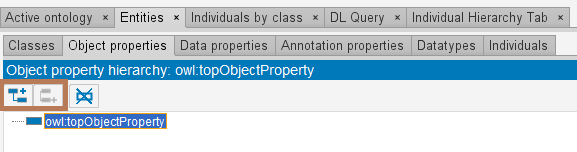
\includegraphics[scale=0.6]{Figures/Protege/CreateObjProp_1.png}
        \caption{Crear una propiedad de objeto}
        \label{CreateObjProp_1}
    \end{figure}

    \item Introducir el nombre de la propiedad.
    \item Seleccionar las opciones que describen las características de la propiedad recién creada (Figura \ref*{CreateObjProp_2})
    \begin{figure}[H]
        \centering
        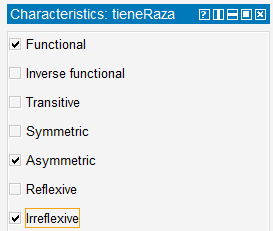
\includegraphics[scale=0.6]{Figures/Protege/CreateObjProp_2.png}
        \caption{Seleccionar características de la propiedad creada}
        \label{CreateObjProp_2}
    \end{figure}

    \item Seleccionar el dominio de la propiedad. Para ello pulsamos sobre el símbolo “+” que se encuentra a la altura de 
    \textit{Domains (intersection)} (Figura \ref*{CreateObjProp_2}).
    \begin{figure}[ht]
        \centering
        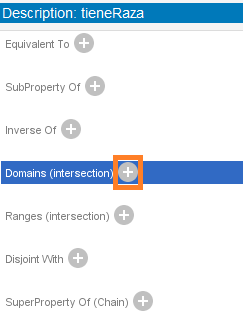
\includegraphics[scale=0.6]{Figures/Protege/CreateObjProp_3.png}
        \caption{Pulsar sobre el símbolo “+” de \textit{Domains (intersection)}}
        \label{CreateObjProp_3}
    \end{figure}

    \item Seleccionar la clase que representa el dominio de la propiedad. Para ello, basta con navegar por la 
    jerarquía que se muestra en la ventana emergente (Figura \ref*{CreateObjProp_4}), elegir la clase correspondiente 
    y pulsar el botón \textit{Aceptar}.

    \begin{figure}[H]
        \centering
        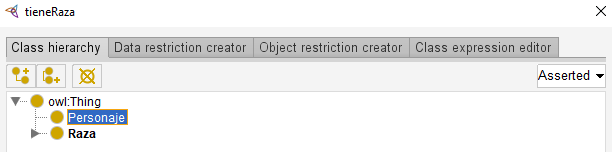
\includegraphics[scale=0.6]{Figures/Protege/CreateObjProp_4.png}
        \caption{Seleccionar clase de dominio}
        \label{CreateObjProp_4}
    \end{figure}

    \item Seleccionar el rango de la propiedad. Para ello pulsamos sobre el símbolo “+” que se encuentra a la altura de 
    \textit{Range (intersection)} (Figura \ref*{CreateObjProp_5}).
    \begin{figure}[ht]
        \centering
        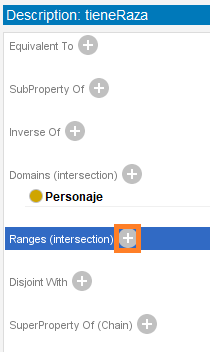
\includegraphics[scale=0.6]{Figures/Protege/CreateObjProp_5.png}
        \caption{Pulsar sobre el símbolo “+” de \textit{Range (intersection)}}
        \label{CreateObjProp_5}
    \end{figure}

    \item Seleccionar la clase que representa el rango de la propiedad. Para ello, basta con navegar por la 
    jerarquía que se muestra en la ventana emergente (Figura \ref*{CreateObjProp_6}), elegir la clase correspondiente 
    y pulsar el botón \textit{Aceptar}.

    \begin{figure}[H]
        \centering
        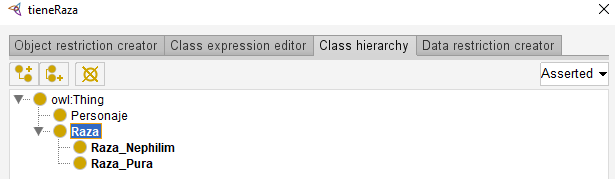
\includegraphics[scale=0.6]{Figures/Protege/CreateObjProp_6.png}
        \caption{Seleccionar clase de rango}
        \label{CreateObjProp_6}
    \end{figure}
\end{enumerate}
Como se puede observar en la figura \ref*{CreateObjProp_6} es posible seleccionar cualquier clase de la jerarquía. En el 
caso de que la clase seleccionada disponga de subclases, éstas también formarán parte del dominio o del rango de la propiedad.\medskip

\subsubsection{Crear una propiedad de datos}\label{CreateDataProp}
Una propiedad de datos se genera prácticamente de la misma forma que una de objetos, con algunas diferencias en lo referente 
a las características y la descripción de la propiedad. 

\begin{itemize}
    \item Si la propiedad no es referente al personaje, contiene el nombre del elemento de dominio y el tipo de valor 
    (ejemplo: Desventaja\_Límite).
    \item En caso contrario, la propiedad debe nombrarse \textit{Per\_Propiedad} (ejemplo: Per\_Nivel).
    \item Si hacen falta varias palabras, separarlas utilizando guiones bajos (ejemplo: Per\_Acum\_Ki).
\end{itemize}

El ejemplo en este caso será la propiedad \textit{Per\_Nivel}, que es 
la propiedad que asocia a un personaje con su nivel:

\begin{enumerate}
    \item Acceder al campo \textit{Entities}, y dentro de este seleccionar la pestaña \textit{Data Properties}.
    \item Seleccionar una propiedad de objeto dentro de la jerarquía de propiedades.
    \item Pulsar uno de los botones que permiten crear propiedades, en función de si deben estar en el mismo nivel jerárquico o 
    en uno inferior, de la misma forma que se indica en los apartados \nameref{CreateSiblingClass} y \nameref{CreateSubclass}
    respectivamente (Figura \ref*{CreateDataProp_1}).
    
    \begin{figure}[H]
        \centering
        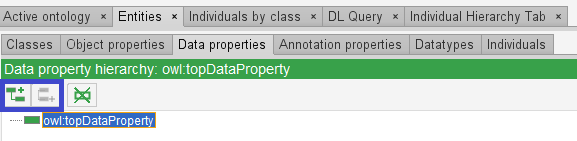
\includegraphics[scale=0.6]{Figures/Protege/CreateDataProp_1.png}
        \caption{Crear una propiedad de objeto}
        \label{CreateDataProp_1}
    \end{figure}

    \item Introducir el nombre de la propiedad.
    \item Indicar si la propiedad es funcional (Figura \ref*{CreateDataProp_2})
    \begin{figure}[H]
        \centering
        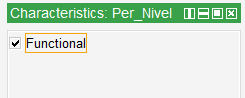
\includegraphics[scale=0.6]{Figures/Protege/CreateDataProp_2.png}
        \caption{Seleccionar características de la propiedad creada}
        \label{CreateDataProp_2}
    \end{figure}

    \item Seleccionar el dominio de la propiedad. Para ello pulsamos sobre el símbolo “+” que se encuentra a la altura de 
    \textit{Domains (intersection)} (Figura \ref*{CreateDataProp_3}).
    \begin{figure}[ht]
        \centering
        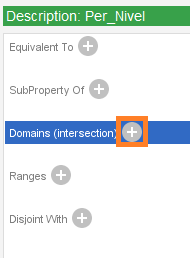
\includegraphics[scale=0.6]{Figures/Protege/CreateDataProp_3.png}
        \caption{Pulsar sobre el símbolo “+” de \textit{Domains (intersection)}}
        \label{CreateDataProp_3}
    \end{figure}

    \item Seleccionar la clase que representa el dominio de la propiedad. Para ello, basta con navegar por la 
    jerarquía que se muestra en la ventana emergente (Figura \ref*{CreateDataProp_4}), elegir la clase correspondiente 
    y pulsar el botón \textit{Aceptar}.

    \begin{figure}[ht]
        \centering
        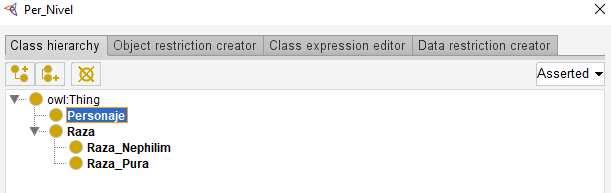
\includegraphics[scale=0.6]{Figures/Protege/CreateDataProp_4.png}
        \caption{Seleccionar clase de dominio}
        \label{CreateDataProp_4}
    \end{figure}

    \item Seleccionar el rango de la propiedad. Para ello pulsamos sobre el símbolo “+” que se encuentra a la altura de 
    \textit{Ranges} (Figura \ref*{CreateDataProp_5}).
    \begin{figure}[H]
        \centering
        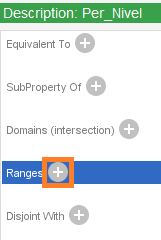
\includegraphics[scale=0.6]{Figures/Protege/CreateDataProp_5.png}
        \caption{Pulsar sobre el símbolo “+” de \textit{Range (intersection)}}
        \label{CreateDataProp_5}
    \end{figure}

    \item Seleccionar el tipo de valor que puede tener esta propiedad. Para ello, basta con pulsar en la opción 
    \textit{Built in datatypes} que se muestra en la ventana emergente (Figura \ref*{CreateDataProp_6}), elegir 
    el tipo de dato más adecuado para la propiedad y pulsar el botón \textit{Aceptar}.

    \begin{figure}[ht]
        \centering
        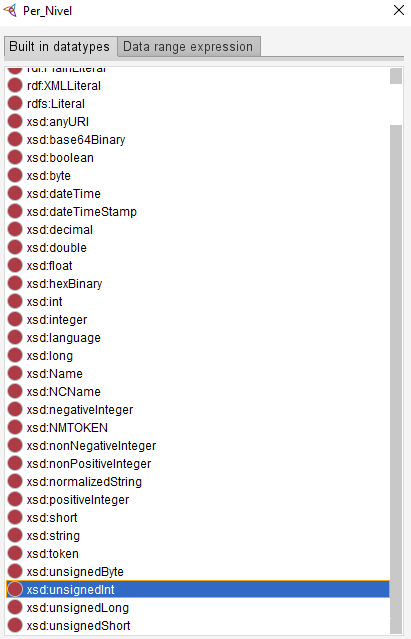
\includegraphics[scale=0.6]{Figures/Protege/CreateDataProp_6.png}
        \caption{Seleccionar clase de rango}
        \label{CreateDataProp_6}
    \end{figure}
\end{enumerate}

\subsection{Individuos}
\protege tiene dos vistas para trabajar con los individuos de la ontología:
\begin{itemize}
    \item Utilizar la opción \textit{Individuals} de la sección \textit{Entities}.
    \item Hacer uso de la opción \textit{Individuals by Class}.
\end{itemize}
El equipo de desarrollo recomienda la segunda opción, ya que permite visualizar la jerarquía de clases y 
contemplar los individuos que forman parte de cada clase.

\subsubsection{Crear un individio de una clase}
Una vez se han definido las clases de la ontología, es hora de crear los individuos que forman parte de cada clase.
Como ejemplo se utilizará el individuo que representa una de las razas \textit{Nephilim} de \anima: \textit{\textbf{Nephilim Sylvain}}.

\begin{enumerate}
    \item Seleccionar la clase a la que se quiere añadir el individuo (Figura \ref*{CreateIndividual_1}).
    \begin{figure}[H]
        \centering
        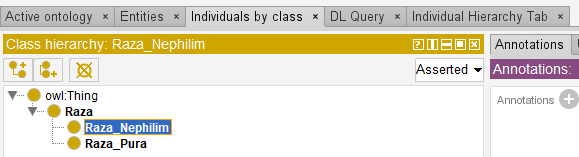
\includegraphics[scale=0.6]{Figures/Protege/CreateIndividual_1.png}
        \caption{Seleccionar la clase a eliminar}
        \label{CreateIndividual_1}
    \end{figure}

    \item Pulsar el botón \textit{Add individual} (Figura \ref*{CreateIndividual_2}).
    \begin{figure}[H]
        \centering
        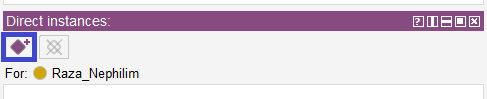
\includegraphics[scale=0.6]{Figures/Protege/CreateIndividual_2.png}
        \caption{Seleccionar la clase a eliminar}
        \label{CreateIndividual_2}
    \end{figure}

    \item Introducir el nombre del individuo (Figura \ref*{CreateIndividual_3}).
    \begin{figure}[H]
        \centering
        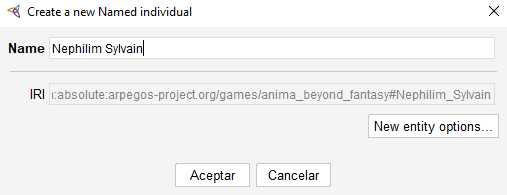
\includegraphics[scale=0.6]{Figures/Protege/CreateIndividual_3.png}
        \caption{Seleccionar la clase a eliminar}
        \label{CreateIndividual_3}
    \end{figure}

    \item Introducir la descripción del individuo en la anotación correspondiente (Figura \ref*{CreateIndividual_4}).
    \begin{figure}[H]
        \centering
        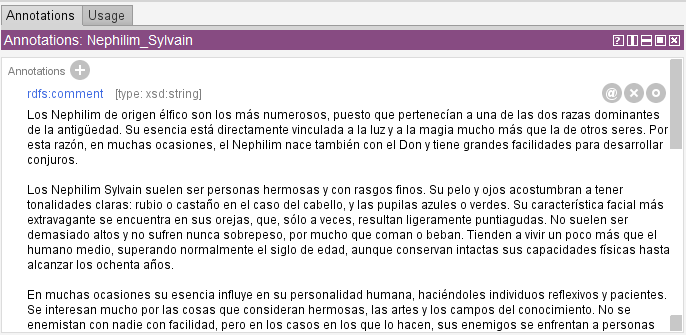
\includegraphics[scale=0.6]{Figures/Protege/CreateIndividual_4.png}
        \caption{Seleccionar la clase a eliminar}
        \label{CreateIndividual_4}
    \end{figure}
\end{enumerate}

\subsubsection{Añadir propiedades a un individuo}
Un individuo se define por las propiedades que lo caracterizan. En este apartado se mostrará cómo se pueden vincular propiedades 
a un individuo, usando como ejemplo un individuo al que llamaremos \textit{TestCharacter}, que representará a un individuo 
de la clase \textit{Personaje} previamente creada, al que se vincularán las propiedades de objeto y dato \textit{tieneRaza} y 
\textit{Per\_Nivel} respectivamente:

\begin{enumerate}
    \item Acceder a la opción \textit{Individuals by Class}.
    \item Buscar la clase \textit{Personaje} en la jerarquía
    \item Crear el individuo \textit{TextCharacter}.
    \item Añadir una aserción de propiedad de objeto. Para ello pulsamos sobre el símbolo “+” que se encuentra a la altura de 
    \textit{Object property assertions} (Figura \ref*{AddProperties_1}).
    \begin{figure}[ht]
        \centering
        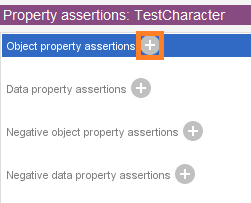
\includegraphics[scale=0.6]{Figures/Protege/AddProperties_1.png}
        \caption{Pulsar sobre el símbolo “+” de \textit{Object property assertions}}
        \label{AddProperties_1}
    \end{figure}

    \item Introducir el nombre de la propiedad en el cuadro de texto de la izquierda (Figura \ref*{AddProperties_2})
    \begin{figure}[ht]
        \centering
        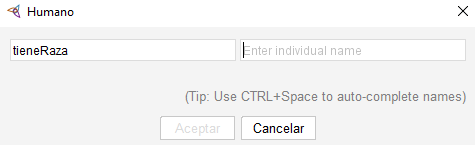
\includegraphics[scale=0.6]{Figures/Protege/AddProperties_2.png}
        \caption{Introducir nombre de la propiedad de objeto}
        \label{AddProperties_2}
    \end{figure}

    \item Introducir el nombre del individuo que se desea relacionar en el cuadro de texto de la derecha (Figura \ref*{AddProperties_3})
    \begin{figure}[ht]
        \centering
        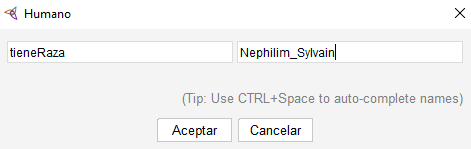
\includegraphics[scale=0.6]{Figures/Protege/AddProperties_3.png}
        \caption{Introducir individuo destino}
        \label{AddProperties_3}
    \end{figure}

    \item Pulsar el botón \textit{Aceptar}.

    \item Añadir una aserción de propiedad de datos. Para ello pulsamos sobre el símbolo “+” que se encuentra a la altura de 
    \textit{Data property assertions} (Figura \ref*{AddProperties_4}).
    \begin{figure}[ht]
        \centering
        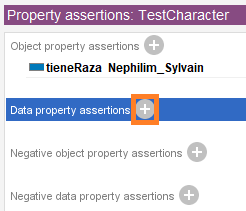
\includegraphics[scale=0.6]{Figures/Protege/AddProperties_4.png}
        \caption{Pulsar sobre el símbolo “+” de \textit{Data property assertions}}
        \label{AddProperties_4}
    \end{figure}

    \item Seleccionar la propiedad que se desea utilizar en la jerarquía de la zona izquierda de la ventana emergente 
    (Figura \ref*{AddProperties_5}).
    \begin{figure}[ht]
        \centering
        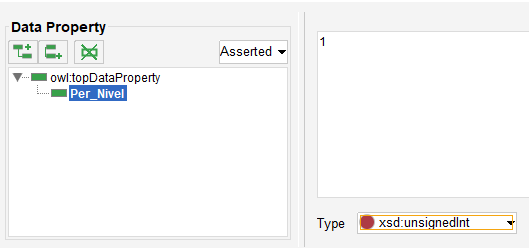
\includegraphics[scale=0.6]{Figures/Protege/AddProperties_5.png}
        \caption{Seleccionar propiedad de datos}
        \label{AddProperties_5}
    \end{figure}

    \item Introducir el valor deseado en el campo de texto de la derecha.
    \item Seleccionar el tipo de dato en el selector \textit{Type}.
    \item Pulsar el botón \textit{Aceptar.}

\end{enumerate}

\subsubsection{Eliminar un individuo}
De igual forma que es posible eliminar una clase, es posible eliminar un individuo. Al igual que en el caso de las clases, 
basta con seleccionar el individuo que se desea eliminar y pulsar el botón \textit{DeleteIndividual} (Figura \ref*{DeleteIndividual}).

\begin{figure}[H]
    \centering
    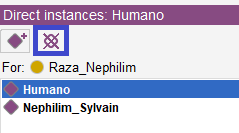
\includegraphics[scale=0.6]{Figures/Protege/DeleteIndividual.png}
    \caption{Seleccionar el individuo a eliminar y pulsar el botón \textit{Delete Individual}}.
    \label{DeleteIndividual}
\end{figure}
